\documentclass[midd]{thesis}

\usepackage{graphicx}
\usepackage{times}
\usepackage{url}
\usepackage{listings}

\lstset{basicstyle=\ttfamily\footnotesize,breaklines=true}

\graphicspath{ {images/} }

\bibliographystyle{plain}

\title {MiddGuard}

\author {Dana Silver}
\adviser {Professor Christopher Andrews}

\begin{document}

\maketitle

\begin{abstract}
Your abstract goes here.
\end{abstract}

\begin{acknowledgements}
Your acknowledgements go here.
\end{acknowledgements}

\contentspage
\tablelistpage
\figurelistpage

\normalspacing \setcounter{page}{1} \pagenumbering{arabic}

\chapter{Introduction}

Be able to create bespoke visualizations quickly.

\section{Visual Analytics}
\begin{enumerate}
  \item Why this is a useful tool in the context of visual analytics.
\end{enumerate}

\chapter{Background}

\section{State of the Art}
  \begin{enumerate}
    \item Tools that currently exist and inspired MiddGuard.
    \begin{enumerate}
      \item Improvise
      \item Eagle Eyes
    \end{enumerate}
  \end{enumerate}

\section{Previous Work on MiddGuard}
\subsection{VAST 2014}

Initial work on the MiddGuard framework began during summer 2014 as a research
project conducted by Christopher Andrews and Dana Silver. For a VAST 2014 Mini-Challenge
2 \cite{vast2014mc2} submission, we created a web interface to
visualize and analyze data from the challenge scenario. Data were preprocessed
using several disjoint Python scripts and the resulting manipulations were
persisted to a SQLite database. On the back-end of the web service, a simple
RESTful Python web server implemented with Flask \cite{flask} and Flask RESTful
\cite{flask-restful} queried the database and transformed data for various
front-end visualizations. The server also performed manipulations in addition
those in the preprocessing stage on a request-by-request basis based on analyst
input in the interactive visualizations.

An example of the flow between preprocessing scripts, back-end server, and
front-end visualization is how we identified points of interest in the
Mini-Challenge 2 geographical data. The VAST 2014 Challenge \cite{vast2014}
posited the following fictitous scenario:

\begin{quote}

In January, 2014, the leaders of GAStech are celebrating their new-found fortune
as a result of the initial public offering of their very successful company. In
the midst of this celebration, several employees of GAStech go missing. An
organization known as the Protectors of Kronos (POK) is suspected in the
disappearance, but things may not be what they seem.

\end{quote}

Available data for Mini-Challenge 2 included vehicle tracking data from
company cars, an ESRI shapefile of the island where GAStech is located, and an
illustrated tourist map of the island. Tracking data contained lists of
latitude, longitude, timestamp, and car ID. A preprocessing script iterated
through each trace's points, identified periods where a car was stopped for
greater than 120 seconds, and saved that coordinate as a destination for the
associated car. A visualization used TopoJSON \cite{topojson-spec} generated
from the shapefile and the tracking data to draw a map of the city overlayed
with cars' movements and destinations. By selecting a destination in the
visualization, an investigator could create a point of interest based on the
names of locations in the tourist map and persist the association of point of
interest and destination to the database. During the persistence step other
destinations within a certain radius would also be associate with that point of
interest.

The VAST 2014 submission was unsuccessful. Working on the tool described above
took most of the available time and investigators were not left with sufficient
time to complete the investigation and write up the results.

The first version of MiddGuard, which was developed in response to summer
research at Middlebury, attempted to generalize parts of the web server and
front-end that could be reused throughout multiple investigations, while keeping
the framework unopinionated with respect to the data it could handle. The
framework's primary features were automatic persistence to a database, data
transport between the server and connected web clients in real-time, centralized
data storage in the web browser, and visualization module loading/unloading in
the browser.

This version of MiddGuard achieved flexibility by automatically loading three
types of customizable packages. These were referred to as analytics, modules,
and models. Analytics were scripts that could be triggered by a remote procedure
call from a front-end visualization. They could be passed data from the
front-end. Using the VAST 2014 example, they were meant to handle computations
like finding other destinations near a point of interest.

Modules were front-end visualizations. JavaScript and CSS files required for the
visualization were declared in a package's \texttt{manifest.json} file. The
database was accessible on the front-end, with each table represented by a
Backbone.js collection. Modules could access collections using the global
\texttt{middguard.entities} object. Collections were updated in real-time over
WebSockets, so by listening to changes in a collection or the models it
contained, a visualization could update in real-time based on changing data on
the server. By extending a base MiddGuard View \cite{backbone} and registering
with MiddGuard by calling a function \texttt{middguard.module(name,
constructor)}, visualizations could be loaded and unloaded from the window with
a button click from MiddGuard's sidebar.

Models were the final piece of customization, intended to give the database
flexible schema to work with any data. Models were a combination of database
migrations and a Bookshelf.js \cite{bookshelf} model declaration. MiddGuard
included a \texttt{migrate} command to migrate models on a table-by-table basis,
applying the results a single database. The model declarations were patched to
emit WebSocket events on create, read, update, and delete events so that
analytics packages could be written to use the models, persist changes, and
communicate those changes to connected clients without needing to explicitly
alert connected clients. Relationships could be established between models using
a special \texttt{relationship} table that stored pairs of table names and row
ids.

\subsection{View Reference Counting}

\begin{enumerate}
  \item MiddGuard Version 1 (Summer 2014)
  \begin{enumerate}
    \item Reusable components
    \item Award/VAST 2015 challenge
  \end{enumerate}
\end{enumerate}


\chapter{Implementation}

\section{Concepts}

\subsection{Data-flow Programming}

At the core of MiddGuard is a data-flow model meant to formalize the analytic
process. The highest unit of abstraction for the data-flow model is a graph.
Analysts can create named graphs from the ``Graphs'' panel in MiddGuard's
sidebar by focusing the ``Graph name'' input, entering a name, and clicking
``Create''. The new graph immediately appears in the list of graphs below the
input for the client who created it and for all other connected clients.
Clicking the graph opens a graph editor specific to the selected graph. Multiple
editors can be open at once, with the editors stacking on the screen to the
right. Figure \ref{fig:sidebar} shows the sidebar with the ``Graphs'' panel in
view and multiple graphs already created and listed below the new graph input.

\begin{figure}[!ht]
  \centering
  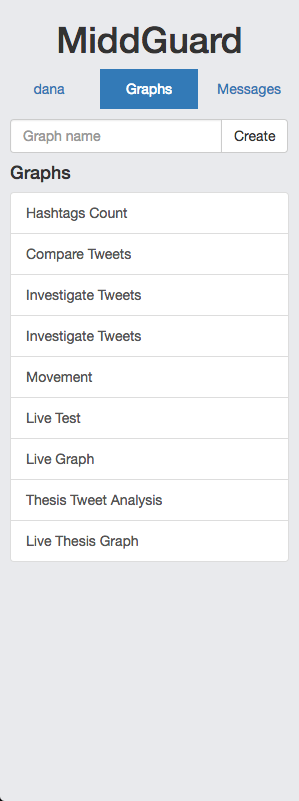
\includegraphics[width=0.5\textwidth]{sidebar-graphs-panel}
  \caption{MiddGuard's built-in sidebar with the ``Graphs'' panel in view.}
  \label{fig:sidebar}
\end{figure}

Graphs are made up of nodes and edges that connect the nodes. In MiddGuard's
vocabulary, these are called nodes and connections. Nodes are instantiated from
modules, by clicking on one of the modules listed in the left panel of the graph
editor. A sample list of modules in this configuration can be seen in figure
\ref{fig:grapheditor}. Modules are discussed further in the subsection on
extensibility.

Nodes are at the heart of the data-flow model's implementation. In this section
we will address the implementation of analytic nodes, seen with blue outlines in
figure \ref{fig:grapheditor}. Visualization nodes and their differences with
respect to analytic nodes will be addressed in the subsequent section on
visualization nodes.

Each node is representative of a function, called the handler, and the node's
dynamically generated context. The handler is a function exposed by the node's
backing module that performs a data transformation. Each nodes' respective
context has an input and an output component. In terms of inputs, the context is
a mapping from the names a node gives its own inputs to names of the outputs of
its incoming connections. For a node's output, the context is a mapping from a
generically named variable, \texttt{output}, to a specifically named table in
the database.

A node's inputs work at two levels, input groups and column-level connections. A
set of column-level connections is encompassed by an input group. Input groups
work at the table level, making a configuration based connection between two
tables in the database. The column-level connections map columns in an output
table to columns in an input table.

Each node has a corresponding table in the database. A mapping from an input
group to an output node creates a mapping from the name the input node (the
owner of the input group) has given that group to the table represented by the
output node. Within each input group are several column mappings, also mapped
from the names of input columns given by the input node to the names of columns
in the output node's table.

The connections generated within the graph editor are stored in MiddGuard's
table of nodes, as a JSON string in the same row as their corresponding input
node. Listing \ref{lst:connectionjson} shows an example connection configuration
for one of the ``Time by Day/Hour'' nodes in the figure \ref{fig:grapheditor}.
The connections for ``Time by Day/Hour'' only have one input group, called
``tweets'', which is connected to the output node with id \texttt{9}. Node
\texttt{9} is the ``@DanaRSilver'' node. The \texttt{output\_node} field serves
as a foreign key referencing another row in the same table. Also stored within
the input group are the column-level connections between the input group and
output node \texttt{9}. These are stored in an array of objects called
\texttt{connections}. Each object within the \texttt{connections} array has an a
key \texttt{input} and a key \texttt{output}. The value of \texttt{input} is the
name the input node has given to the column and the value of \texttt{output} is
the name the output node has given to the column.

\begin{lstlisting}[caption={A node's connection configuration. The node has a connection from its input group ``tweets'' to the node with id 9.}, captionpos=b, label={lst:connectionjson}]
{
  "tweets": {
    "output_node": 9,
    "connections": [
      {
        "output": "handle",
        "input": "handle"
      },
      {
        "output": "tweet",
        "input": "tweet"
      },
      {
        "output": "timestamp",
        "input": "timestamp"
      }
    ]
  }
}
\end{lstlisting}

We considered multiple factors when deciding how to store nodes and their
connections in the database before deciding on a JSON string stored with the
connections' input node. We wanted a storage method that was portable,
efficient, and convenient. Portability meant that we could easily export the
configuration of nodes and connections to a text file so they could be read back
in and the graph could be reassembled in a different system. Efficiency was
determined by the number of database operations required to access the
configuration. This was important since we have to read and write connections
whenever a node is accessed or modified in the graph editor. Convenience meant
that it was not overly complex to access and modify the connections from a
programming perspective.

In addition to the JSON string storage method we implemented, we considered
storing connections and nodes in separate tables, with either each column-level
connection in its own row or each group of column-level connections in a row.
The former performed no grouping amongst column mappings, while the latter
grouped each input group's columns in a single row.

The first option (each column mapping has its own row) was appealing since it
took advantange of the relational database, using foreign keys to associate
column mappings with their nodes. However, this method is less portable since it
requires multiple steps to export all the node information and their associate
column mappings from the database to a structured text file. It is also less
efficient since it requires reading a row from the database for every column
mapping, in addition to a row for every node. Finally, it would be less
convenient to develop with because it would require more queries to the database
to obtain all the information to construct the graph than if we stored the
connection information close to the nodes.

For similar reasons, we ruled out the second option of storing all column level
connections in a row, grouped by their input group. This seemed like a poor
compromise between storing all column mappings separately and storing all
connection information with their nodes. We would lose the elegance of
conforming to the facilities of a relational database, and still have to query
the database multiple times to assemble a graph or export/import the data.

The implemented method of storing a node's connection in the same database table
row as the node, in a JSON string, satisfied all our requirements. It is
portable: JSON is common format to export human readable configuration. We can
simply query all nodes and write out their metadata and JSON string as
connections. It is efficient to access nodes and connections to construct a
graph. All of a graph's nodes and connections can be accessed by reading
\textit{n} rows from the database, where \textit{n} is the number of nodes in a
graph. It is convenient to work with this format, since all the connection data
for a node can be obtained by calling JavaScript's built-in \texttt{JSON.parse}
method on a node's connections column.

A node's connections can be edited in the graph editor until runtime, when a
node's handler funtion is executed. At this point, MiddGuard makes a query for
the node in the database and retrieves its stored connections. Parsing the
connections JSON string lets MiddGuard access the mapping of input groups to
output nodes and the mappings of column names between nodes. MiddGuard makes
additional queries to determine the table names of connected output nodes. With
just this information, MiddGuard can construct the dynamically generated context
to pass into the handler function. Listing \ref{lst:nodecontext} is a sample of
the context passed into one of the ``Time by Day/Hour'' nodes visible in figure
\ref{fig:grapheditor}. At the top level it includes \texttt{inputs} and
\texttt{table}. \texttt{inputs} is an object mapping each of the nodes input
groups to data about the connected output node. Within \texttt{inputs} are:
\texttt{knex}, an instance of the Knex.js SQL generator \cite{knexjs}, used to
access the table connected to an input group; \texttt{cols}, the column-level
mapping between the node's input group and the connected output node's column
names; and \texttt{tableName}, the name of the connected output node's table
name. \texttt{cols} and \texttt{tableName} are meant to give access to the
information available for more advanced queries, such as table joins.

The other top-level key in the context, \texttt{table}, gives access to the
output table for this node. Like each input group in \texttt{inputs}, it has a
\texttt{knex} accessor to generate SQL to query the database, and a
\texttt{name}, which is the node's own table name. \texttt{table} doesn't need a
column mapping, since the column names are the same as the ones the node has
assigned itself as outputs.

\begin{lstlisting}[caption={The context passed into a ``Time by Day/Hour'' node's handler function.}, captionpos=b, label={lst:nodecontext}]
{
  inputs: {
    tweets: {
      knex: [Object],            // database connection instance
      cols: {
        handle: 'handle',
        tweet: 'tweet',
        timestamp: 'timestamp'
      },
      tableName: 'download-tweets-danarsilver_1'
    },
    table: {
      knex: [Object],            // database connection instance
      name: 'aggregate-time_2'
    }
  }
}
\end{lstlisting}

Having to make additional queries to access output nodes' table names is a
potential source of ineffiency not addressed by our connections storage format.
A way around this would be to duplicate the table name each time it appears in a
connections JSON string. We decided against duplicating the data and in favor of
making additional database queries instead to avoid fragmenting the information,
should the table name change. Should we need to update a node's table name, it
can be done once for the row, rather than having to update the connections
string in all other connected nodes.

\begin{figure}[!ht]
  \centering
  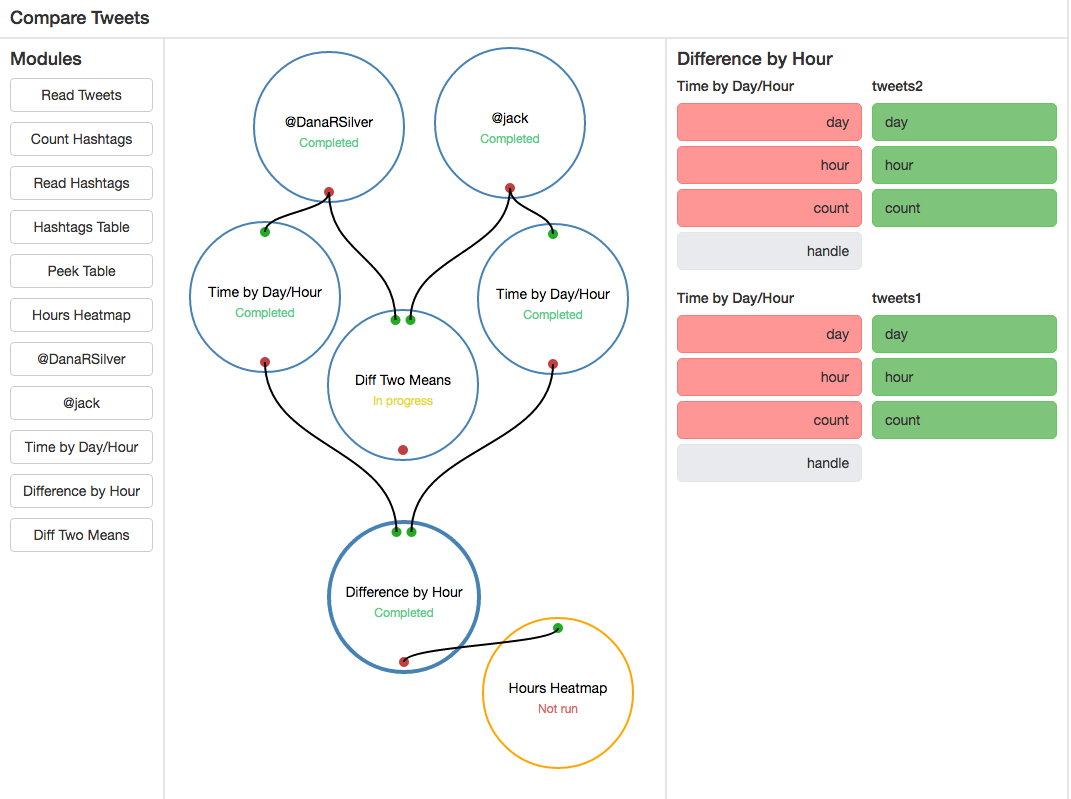
\includegraphics[width=1\textwidth]{compare-tweets-graph-editor-no-sidebar}
  \caption{MiddGuard's graph editor user interface, open on a graph named
  ``Compare Tweets''. On the left, the modules panel lists all loaded modules,
  from which nodes can be created. In the center, the graph editor canvas has
  seven nodes initialized from their respective modules, and connections between
  the nodes. On the right, the detail panel shows the column mappings between
  the ``Difference by Hour'' node and its connections to two
  ``Time by Day/Hour'' nodes.}
  \label{fig:grapheditor}
\end{figure}

\subsection{Visualization Nodes}

Visualization nodes, like analytic nodes, are added from modules in the graph
editor. Figure \ref{fig:grapheditor} has a visualization node with the label
``Hours Heatmap'' with an orange outline. Like analytic nodes, visualization
nodes have input groups that can be connected to output nodes, and column
mappings between the two nodes on the ends of the connections. The primary
difference between analytic nodes and visualization nodes is that the handler
for an analytic node is a single function that is called and run on MiddGuard's
back-end server, while the handler for a visualization node is a newly
instantiated Backbone.js View \cite{backbone} that is rendered in the web
client.

The instantiated view for a visualization node has an instance method called
\texttt{createContext}, which can be called to dynamically generate the context
for a view, just as the MiddGuard generates the context for an analytic node on
the back-end and passes it into the handler function. The context for a
visualization node has the same structure as that of an analytic node, less the
output \texttt{table}, since a visualization node's output is a visualization,
rather than a table of data.

Additionally, the \texttt{knex} key for each input group is replaced with an
instance of a Backbone Collection (with a key aptly named \texttt{connection}),
which can be used like the \texttt{knex} key to access the data from output node
connected to that particular input. MiddGuard instantiates a Backbone collection
for each analytic node and a corresponding endpoint on the back-end to transmit
the analytic node's data to the collection, as required by a visualization node.

A potential improvement in the implementation of visualization nodes would be to
only instantiate collections for analytic nodes that output to visualization
nodes. Other nodes' data will never be accessed, so it is not necessary to
maintain collections on the front-end or the endpoints on the back-end to
transmit data to them. However, this is a low-priority improvement since there
is little overhead in terms of memory usage to create an empty connection on the
front-end or add the event listeners that handle data transmission to Node.js's
event loop on the back-end.

\subsection{Visual Programming}

Visual programming abstracts away the details of the data-flow model within
MiddGuard as descibed in the previous sections, and the independent
implementation details of each node. A major motivation for MiddGuard is to
facilite quick construction of complex visual analytic tools. MiddGuard's system
for visual programming allows investigators to quickly compose data
transformations and visualizations. The visual component creates an expressive
representation of the steps to reproduce a visualization.

The visual programming interface takes place in the three panels of the graph
editor, seen in figure \ref{fig:grapheditor}. The left panel, titled
``Modules'', lists all modules from which nodes can be instantiated. Clicking a
module's button in the list adds a node of that type to the canvas in the middle
panel.

The middle panel's canvas is a free-form space limited by the height of the
window and a 500 pixel width constraint. Nodes, once added to the canvas, are
outlined circles that can be rearranged and connected to one another. Analytic
nodes and visualization nodes are outlined in blue and orange respectively, to
make them easy to differentiate.

Figure \ref{fig:annotatednode} shows an analytic node with all its elements for
user interaction in view. The cross in the upper left corner is used to drag the
node around the canvas. Allowing nodes to be draggable is a simple solution to
problem of node layout. A downside is the additional effort and time required on
the part of the user to position and reposition nodes in the canvas, but this is
outweighed by both its simplicity to implement over a layout algorithm and the
flexibility for the user to customize the graph view as best appeals to their
idea of the investigation.

The ``play'' button, located in the top right of each node abstracts both
analytic and visualization nodes' action. In an analytic node clicking play
calls its handler function. In a visualization node, the play button creates a
new instance of a visualization. Pressing a visualization node's play button
again removes that visualization from the browser window. Like the graph
editors, stack horizontally in the browser window. The user can scroll through
them from left to right.

While web scrolling is typically done vertically, we implemented view layout
horizontally, since MiddGuard was designed to be used on the same system used
for the preliminary VAST 2014 and VAST 2015 investigations. These investigations
used a system of three 27 inch displays arranged side by side
\cite{middguard-dinofunworld}.



An output node can be connected to another node's input group by clicking two of
the red and green circles on different nodes that represent connections. Figure
\ref{fig:annotatednode} shows a node with one green input group circle at the
top of the node and a red output circle at the bottom of the node.

Since each node is backed by a table in MiddGuard's relational database,
connections between two nodes, visualized by a line between one node's output
and another's input, represent data flowing out of one or more nodes' backing
table into another node's table. For example, in figure \ref{fig:grapheditor},
data flows out of the tables for nodes ``@jack'' and ``@dana'' into the table
for the node ``Diff Two Means''.

\begin{figure}[!ht]
  \centering
  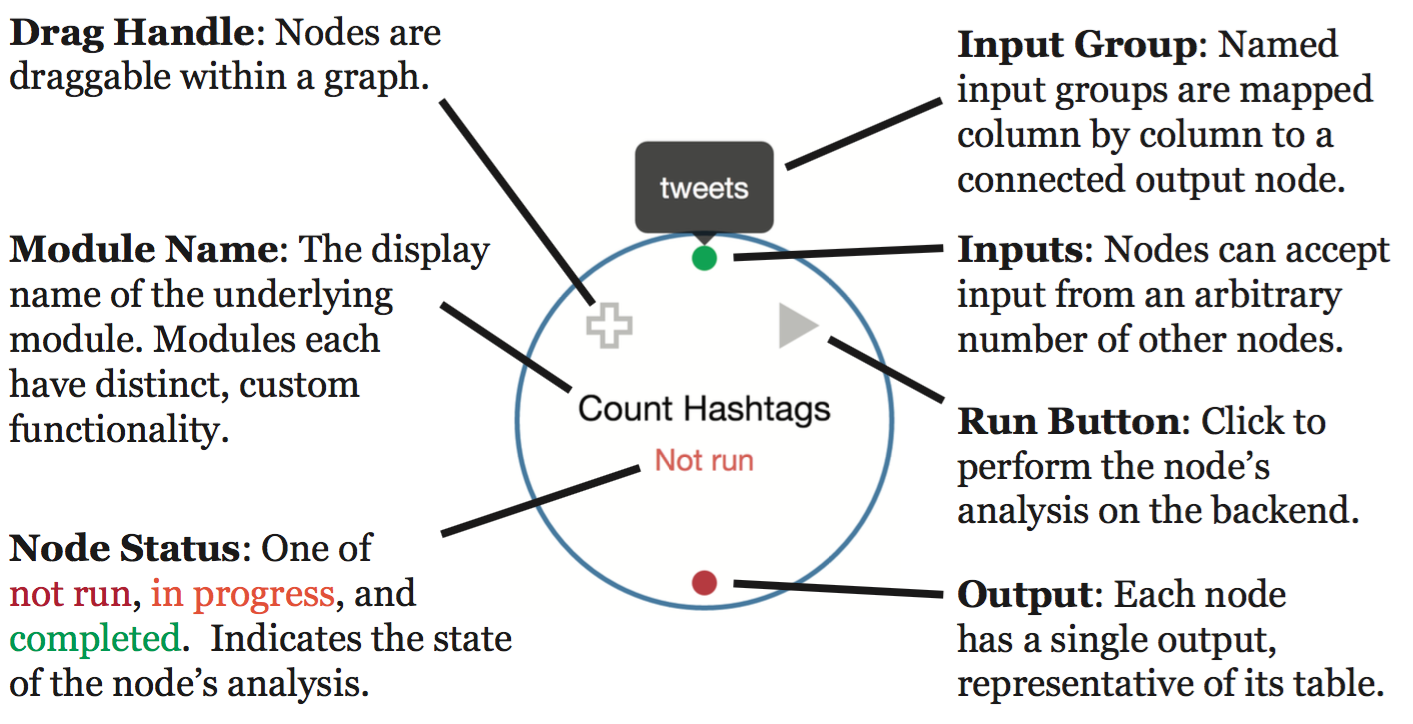
\includegraphics[width=1\textwidth]{middguard-analytic-node-annotated}
  \caption{An analytic node in a graph. Important features are annotated and the
  node's only input group, ``tweets'', is moused over to show its accompanying
  tooltip.}
  \label{fig:annotatednode}
\end{figure}


\section{}
\subsection{Real-time collaboration}

  \begin{enumerate}
    \item Dataflow programming
    \item Visual programming
    \item Collaborative/real-time
    \item Extensibility
    \begin{enumerate}
      \item Front-end views
      \item Back-end analytic nodes
    \end{enumerate}
    \item Reusable nodes (agnostic of input/output data)
    \item Technology choices
  \end{enumerate}

\section{Technology}
  \begin{enumerate}
    \item Node.js
    \item Relational database (instead of NoSQL)
    \item Socket.io
    \item ORM
    \item Backbone.js
  \end{enumerate}

\chapter{Results}
  \begin{enumerate}
    \item Test/example case (tweet analysis)
    \item Ease of use for developer
    \item APIs exposed on front-end and back-end
  \end{enumerate}

\chapter{Discussion}
  \begin{enumerate}
    \item Use in real investigation (VAST Challenge 2016)
    \item Room for improvement
    \begin{enumerate}
      \item Better caching on front-end to help developers optimize DOM/memory
      usage
      \item Have to see if there is any else I don't have time to implement
    \end{enumerate}
  \end{enumerate}

\chapter{Conclusion}
  \begin{enumerate}
    \item Revisit points from previous sections
    \item Why MiddGuard is an important visual analytics tool
    \item Open source prospects
  \end{enumerate}

\appendix
\chapter{Chapter 1 of appendix}
Appendix chapter 1 text goes here

\bibliography{thesis}

\end{document}
